\documentclass[a4paper,12pt]{article}
\usepackage[left=1cm,right=1cm,top=3cm,bottom=3cm,a4paper]{geometry}
\usepackage[pdftex]{graphicx}
\usepackage{amsmath}
\usepackage{amsfonts}
\usepackage{amssymb}
\usepackage{graphicx}
\usepackage{kotex}
\newcommand{\dbar}{d\hspace*{-0.08em}\bar{}\hspace*{0.1em}}
\usepackage[onehalfspacing]{setspace}
\begin{document}
	\begin{flushleft}
		$<$Microcanonical ensemble 다른 식으로 생각해보기 Reif 6.2,6.3절$>$ 
	\end{flushleft}
\paragraph{Heat reservoir에 닿아 있는 계}
교과서 85쪽 그림 6-4를 보자. 아주 큰 계를 $A_{H.R}$ (heat reservoir), 작게 혹처럼 붙어있는 계를 $A$라고 하자. 이 경우는 수영장($A_{H.R}$)에 작은 유리병($A$)이 떠 있는 것으로도 생각할 수 있다. 
$A$는 평형상태에 도달해 어떤 미시상태 $i$에 있고, 에너지 $E_i$를 지니게되었다. 우리가 관심있는 것은 평형상태에서 $A$가 특정 미시상태 $i$에 도달할 확률, $p_i$이다. $A_{H.R}$ 와 $A$ 가 서로 약하게 상호작용하여 둘의 에너지를 서로 더할 수 있다고 하면, 총 에너지 $E_0$은,
$$E_0=E_i+E_{H.R}$$
이다. $A$가 에너지 $E_i$에 있을 때, Heat reservoir $A_{H.R}$은 $E_{H.R}=E_0-E_i$에 가까운 에너지를 가져야 한다. ($\delta E$ 범위 안에서) 그러므로 $A$가 한 미시상태 $i$에 있을 때, 묶인 계 $A_0$의 number of accesible states는 $A_{H.R}$의 그것과 같다.
$$\Omega_0(E_0)=\Omega_{H.R}(E_{H.R},\delta E)=\Omega_{H.R}(E_0-E_i,\delta E)$$ 
통계의 기본 가정에 의해 $A$ 가 $i$ 상태에 있을 확률은 $A_0$의 number of accesible states에 비례할 것이다.
$$p_i=C'\,\Omega_{H.R}(E_0-E_i,\delta E)$$
$C'$은 나중에 normalization 조건인
$$\sum_{i}p_i=1$$
으로 구할 수 있다.
이제 $A_{H.R}$(수영장)이 $A$(유리병)보다 아주 큰 계라는 사실을 이용하겠다. 즉 $E_i \ll E_0$ 이므로, 다음 어림식을 염두에 두고,
$$f(x-\delta x)=f(x)+f^{(1)}(x)(-\delta x)+\frac{f^{(2)}}{2!}(-\delta x)^2+\cdots$$
$\ln\Omega_{H.R}(E_0-E_i)$를 어림하면,
$$\ln \Omega_{H.R}(E_0-E_i)=\ln \Omega_{H.R}(E_0)+\left[ \frac{\partial \ln \Omega_{H.R}}{\partial E_{H.R}}\right]_{E_0} (-E_i)+\cdots$$
가 된다. $E_i\ll E_0$ 이므로 2차 이상의 항은 무시할 수 있다. 한편,
$$\frac{\partial S}{\partial E}=\frac{k_B\,\partial \ln \Omega}{\partial E}=\frac{1}{T}$$ 에서
$$\left[ \frac{\partial \ln \Omega_{H.R}}{\partial E_{H.R}}\right]_{E_0}=\frac{1}{k_B\,T}=\beta $$은 $A$의 에너지 $E_i$에 무관한 값으로, heat reservoir $A_{H.R}$의 에너지가 $E_0$일 때 그것의 온도와 관련있는 값이다. Heat reservoir가 원칙적으로는 온도가 변하지 않으므로 heat reservoir의 $\beta$ 값이 한번 주어진다면 변하지 않는 상수일 것이다. 따라서 어림식을 다시 써보면, 
$$\ln \Omega_{H.R}(E_0-E_i)\sim\ln \Omega_{H.R}(E_0)-\beta E_i$$
$$\Omega_{H.R}(E_0-E_i)\sim\Omega_{H.R}(E_0)\,e^{-\beta E_i}$$
$\Omega_{H.R}(E_0)$ 은 상수이므로, 
$$p_i=C'\,\Omega_{H.R}(E_0-E_i)=C'\,\Omega_{H.R}(E_0)\,e^{-\beta E_i}=C\,e^{-\beta E_i}$$
normalization constant $C$를 결정하려면, 
$$1=\sum_{i}p_i=\sum_{i}Ce^{-\beta E_i}=C\sum_{i}e^{-\beta E_i}$$
$$C=\frac{1}{\sum_{i}e^{-\beta E_i}}$$
따라서,
$$p_i=\frac{e^{-\beta E_i}}{\sum_{i}e^{-\beta E_i}}$$
이때, $e^{-\beta E_i}$를 Boltzmann factor라고 부른다. 
Microcanonical ensemble에서는 계의 에너지는 모두 같은 경우이므로 $$E_i=E,\quad E<H<E+\delta E$$이고, $p_i$는 모두 같다. 
\paragraph{응용하기-상자성(교과서 연습문제 3-1)참고} 단위 부피당 $N_0$의 자기 원자를 갖는 물질을 생각하자. 자기 원자들은 외부 자기장 $\vec{H}$에 놓여 있다. 각 원자는 스핀 1/2과 자기 모멘트 $\mu$를 갖는다고 하자. 각 원자의 자기 모멘트는 외부 자기장 $\vec{H}$에 나란히 또는 거꾸로 배열된다. 물질이 절대온도 $T$에 있다면 이러한 원자의 평균 자기 모멘트 $\bar{\mu}_H$ 는 어떻게 될까? 한 원자를 따로 떼어내서 작은 계 $A$(유리병)으로 다루고, 다른 모든 원자들을 heat reservoir $A_{H.R}$(수영장)로 간주해서 이 물음을 해결할 수 있다. \\
각 원자는 두 가지 상태에 있을 수 있다. 
\begin{center}
1. 스핀이 위로 향하는($\vec{H}$에 나란한) 상태 (+)\\
2. 스핀이 아래로 향하는($\vec{H}$에 거꾸로인) 상태 (-)
\end{center}
(+) 상태에서는 원자의 자기모멘트 $\vec{\mu}$ 가 $H$에 나란하므로 $\mu_H=\mu$ 이고 이에 해당하는 자기 에너지는 $\epsilon_+=-\mu H$ 이다. 따라서 이 상태에 원자가 있을 확률은 다음과 같다. 
$$p_+=Ce^{-\beta \epsilon_+}=Ce^{\beta\mu H}$$ 
(-) 상태에서는 원자의 자기모멘트 $\vec{\mu}$ 가 $H$에 거꾸로 이므로 $\mu_H=-\mu$ 이고 이에 해당하는 자기 에너지는 $\epsilon_-=\mu H$ 이다. 따라서 이 상태에 원자가 있을 확률은 다음과 같다. 
$$p_-=Ce^{-\beta \epsilon_-}=Ce^{-\beta\mu H}$$ 
$\mu $가 양수일 때, $\epsilon_+$가 $\epsilon_-$보다 작기 때문에 $p_+$가 $p_-$보다 크다. ($\beta>0$이므로) 즉 원자가 $\vec{H}$와 나란할 확률이 더 크게 된다. 
$$\begin{cases}p_+=Ce^{\beta\mu H}&\vec{H}\mbox{ 에 나란할 확률 }\\p_-=Ce^{-\beta\mu H} &\vec{H}\mbox{ 에 거꾸로일 확률}
\end{cases}$$
여기서 우리가 생각해야하는 주요 변수는 
$$y=\beta \mu H=\frac{\mu H}{k_B T}$$
로, 특정 열 에너지에 대한 자기 에너지의 비이다. $T$가 매우 크다면 $y$가 매우 작아져서 ($\simeq 0$) $p_+$ 와 $p_-$가 비슷해진다. 즉 온도가 아주 커지면 $\mu$의 방향이 완벽하게 random해져서 $\bar{\mu}_{H}\simeq0$ 이다. 반면에 $T$가 아주 작다면 $y$가 매우 커져서 $p_+$가 $p_-$보다 훨씬 커진다. 즉 온도가 낮아지면 $\bar{\mu}_{H}\simeq\mu$이다. 이것을 실제로 계산해 볼 수도 있다. 
$$\bar{\mu}_H=\frac{p_+\mu+p_-(-\mu)}{p_++p_-}=\mu\frac{e^{\beta\mu H}-e^{-\beta\mu H}}{e^{\beta\mu H}+e^{-\beta\mu H}}=\mu \tanh \beta\mu H=\mu\tanh\frac{\mu H}{k_BT}$$
사실 이 결과는 교과서 연습문제 3-1 에서 본 적이 있다. (정확히는 3-1번 문제 (다)번으로 답은 $E=-\mu HN\tanh\frac{\mu B}{k_BT}$로 나왔다.)
단위 부피당 평균 자기 모멘트 혹은 Magnetization $\bar{M}_0$은 ($\mu$가 $H$에 나란할 확률이 더 높으므로) $H$의 방향과 나란하고, 크기는 $$\bar{M}_0=N_0\bar{\mu}_H$$이다.
$\tanh$ 함수의 어림을 이용해서 앞서 했던 논의를 확인해보자.
\begin{flushleft}
	$y\ll1$ 일 때, $\tanh y=y$\\
	$\mu H/k_BT\ll 1$일 때, $\tanh \mu H/k_BT=\mu H/k_B T$
	$$\therefore\bar{\mu}_H=\frac{\mu^2H}{k_BT}, \quad \bar{M}_0=N_0\bar{\mu}_H=\frac{N_0\mu^2}{k_BT}H=\chi H$$
$\chi$를 magnetic susceptibility라고 부르고 절대온도에 반비례한다.(Curie의 법칙)\\
	$y\gg1$ 일 때, $\tanh y=1$\\
	$\mu H/k_BT\gg 1$일 때, $\tanh \mu H/k_BT=1$
	$$\therefore\bar{\mu}_H=\mu,\quad \bar{M}_0=N_0\bar{\mu}_H=N_0\mu\mbox{ (independent of }H)$$
\end{flushleft}	
마지막으로 $$\bar{M}_0=N_0\bar{\mu}=\mu N_0\tanh{\frac{\mu H}{k_BT}}, \quad \frac{\bar{M}_0}{\mu N_0}=\tanh\frac{\mu H}{k_B T}$$ 에서 $\bar{M}_0/\mu N_0$ 의 $\mu H/k_BT$에 대한 그림을 그려보면 다음과 같다. 
	\begin{figure}[h]
	\centering
	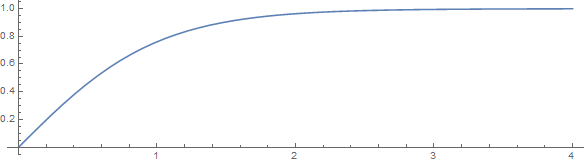
\includegraphics[width=0.8\columnwidth]{fig1.png}
	\caption{온도 T, 자기장 H에 대한 magnetization의 의존성}
\end{figure}
\end{document} 